\documentclass{article}
\usepackage{graphicx} % Required for inserting images
\usepackage{float}
\usepackage{amsmath}
\title{Lesson 13 Homework - Proof Writing}
\author{William Wang}
\date{November 2025}

\begin{document}

\maketitle
\section{}
\textbf{Surface:}
\[
x^2 - y^2 = z^2.
\]

\text{(a) Cross-section in the $xy$-plane ($z=0$).}
\[
x^2 - y^2 = 0 
\quad\Longrightarrow\quad
(x-y)(x+y)=0
\]
\[
\text{Cross-section: } y = x,\; y=-x.
\]
Should look like an X
\text{(b) Cross-section in the $yz$-plane ($x=0$).}
\[
0 - y^2 = z^2
\quad\Longrightarrow\quad
-y^2 = z^2.
\]
\[
\text{Only solution: } y=0,\;z=0.
\]
A singular point
\text{(c) Cross-section in the $xz$-plane ($y=0$).}
\[
x^2 = z^2
\quad\Longrightarrow\quad
z = \pm x.
\]
\[
\text{Cross-section: } z=x,\; z=-x.
\]
A big circle
\text{(d)}
\begin{figure}[H]
    \centering
    
\includegraphics[width=0.5\linewidth]{1.png}

\end{figure}
\begin{figure}[H]
    \centering
    
\includegraphics[width=0.5\linewidth]{2.png}
\end{figure}
\begin{figure}[H]
    \centering
    
\includegraphics[width=0.5\linewidth]{3.png}
 
\end{figure}

\text{(e) Most helpful cross-sections.}

For fixed $x=a$:
\[
a^2 - y^2 = z^2
\quad\Longleftrightarrow\quad
y^2 + z^2 = a^2,
\]
which are circles of radius $|a|$.  
Planes containing the $x$-axis  give:
\[
z=\pm x.
\]

Thus the most informative cross-sections are:
Slices $x=a$, which give circles.
Any plane through the $x$-axis, which gives lines $z=\pm x$.
\section{}
\subsection{}
Its a sphere!
\begin{figure}
    \centering
    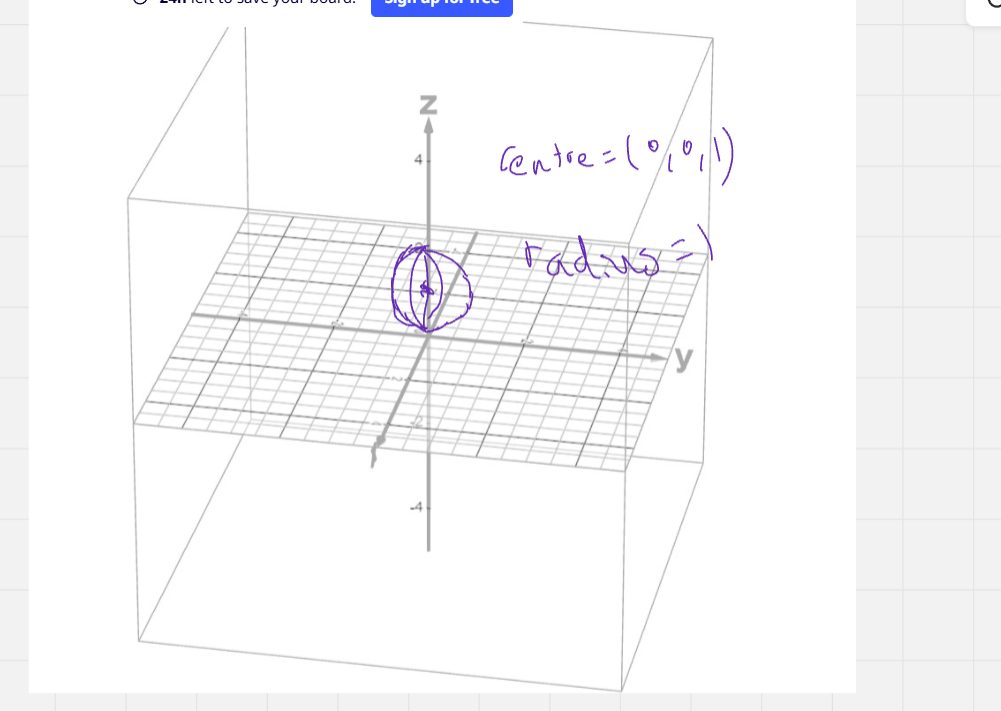
\includegraphics[width=1\linewidth]{4.png}
\end{figure}
\subsection{}
Since we know that $r^2 = x^2 + y^2$, then we can sub in this value to get 
\[x^2+y^2+z^2=2z\]
Then using Simon's Favourite Factoring Trick, we can add 1 to both sides and move the $2z$ over to get the square of binomial
\[x^2+y^2+z^2-2z+1=1 \implies x^2+y^2+(z-1)^2 = 1\]
This gives us the standard equation of a sphere with centre $(0,0,1)$ and radius of 1. 
\end{document}
